\documentclass{../preamble}

% Title information
\date{18.01.2021 - 22.01.2021}
\sheetnumber{7}
\version{28. Dezember 2020}

% Document
\begin{document}

\maketitle

\makedisclaimer

\clearpage

\begin{task}[credit = \stars{0}{3}]{Theoriefragen}
    \begin{subtask*}{Grundlegendes}
        \begin{enumerate}
            \item Wie hängen die Begriffe \textcolor{keywordcolor}{throws} und \textcolor{keywordcolor}{throw} zusammen? Wo wird was verwendet?
            \item Ist es sinnvoll, eigene Exceptionklassen zu definieren? Welche Vorteile ergeben sich hieraus?
            \item Nennen Sie die Methoden der \code{Assert}-Klasse, die Sie zum Testen bei einem typischen JUnit Testcase in der Vorlesung  kennengelernt haben, und beschreiben Sie kurz deren Verwendung.
        \end{enumerate}

        \begin{solution}
            \begin{enumerate}

                \item \textcolor{keywordcolor}{throws} wird im Methodenkopf verwendet, um zu signalisieren, dass eine Methode eine Exception dieser Klasse wirft.
                      \newline
                      \textcolor{keywordcolor}{throw} hingegen wird in der Methode verwendet, um eine  \textcolor{keywordcolor}{throw new} Exception() (dabei kann statt Exception auch eine von Exception abgeleitete Klasse stehen). Falls eine \code{Exception} geworfen wird, so wird die momentane Ausführung der Methode unterbrochen. \code{Exception} bieten die Möglichkeit, wenn etwas Ungewöhnliches im Programm geschieht, diese Tatsache von der Hauptlogik eines Programms zu trennen und auf die Ursache des Fehlers zurück zu führen.
                \item Bei eigenen Exception-Klassen können speziellere Informationen an den Konstruktor übergeben werden, was die Fehlerbehandlung erleichtern kann und zum Beispiel für eine detaillierte Ausgabe der Probleme sorgt.
                      \br
                      Ein weiterer Grund für eigene Exception-Klassen ist, dass der Name damit häufig schon die wesentliche Information enthalten kann, z.B. der Name \code{ArrayIndexOutOfBoundsException} sagt zusammen mit dem Call-Stack eigentlich schon alles, was man über den Fehler wissen muss.
                \item
                      \begin{itemize}
                          \item \code{assertEquals}(erwarteter Wert, tatsächlicher Wert, (ggf. Abweichung)):
                                \newline
                                Die Methode gibt einen Fehler, wenn sich die beiden Werte unterscheiden (bzw. wenn sie sich um mehr als die Abweichung unterscheiden)
                          \item \code{assertTrue}(Prädikat/boolescher Wert):
                                \newline
                                Die Methode liefert einen Fehler, wenn die Methode false zurückliefern würde
                          \item \code{assertThrows}(Exceptionname.\textcolor{keywordcolor}{class}, Executable Lambda-Ausdruck): \newline
                                Die Methode liefert einen Fehler, wenn die Exception nicht geworfen wurde
                                \begin{lstlisting}[style = Java]
public interface Executable {
 void execute() throws Throwable;
}
\end{lstlisting}
                                \begin{itemize}
                                    \item Formaler Aufbau einer Executable
                                          \begin{lstlisting}[style = Java]
Executable example = () -> Operationen
\end{lstlisting}
                                \end{itemize}
                      \end{itemize}
            \end{enumerate}
        \end{solution}
    \end{subtask*}

    \clearpage

    \begin{subtask*}{Wahr oder falsch?}
        Welche der folgenden Aussagen ist wahr?
        \begin{enumerate}[label = (\Alph*)]
            \item Auf einen \textcolor{keywordcolor}{try}-Block muss immer mindestens ein \textcolor{keywordcolor}{catch}-Block folgen.
            \item Wenn Sie eine Methode schreiben, die eine Exception auslösen könnte, müssen Sie diesen riskanten Code mit einem \textcolor{keywordcolor}{try}/\textcolor{keywordcolor}{catch}-Block umgeben.
            \item Auf einen \textcolor{keywordcolor}{try}-Block können beliebig viele verschiedene \textcolor{keywordcolor}{catch}-Blöcke folgen.
            \item Eine Methode kann nur eine einzige Art von Exception werfen.
            \item Die Reihenfolge der \textcolor{keywordcolor}{catch}-Blöcke ist grundsätzlich gleich gültig.
            \item Laufzeit (Runtime)-Exceptions müssen gefangen oder deklariert werden.
            \item Es darf kein Code zwischen dem \textcolor{keywordcolor}{try}-Block und dem \textcolor{keywordcolor}{catch}-Block  geschrieben werden.
            \item Eine Methode wirft eine Exception mit dem Schlüsselwort \textcolor{keywordcolor}{throws}.
        \end{enumerate}

        \begin{solution}
            \begin{enumerate}[label = (\Alph*)]
                \item Ein \textcolor{keywordcolor}{try}-Block kommt nie allein, sondern immer mit einem oder manchmal mehreren \textcolor{keywordcolor}{catch}-Blöcken, die unmittelbar danach kommen. Die einzigen Ausnahmen sind, wenn nach einen \textcolor{keywordcolor}{try}-Block ein \textcolor{keywordcolor}{finally}-Block\footnote{Das Schlüsselwort wurde nicht in der Vorlesung behandelt und wird abgeraten es zu verwenden} folgt oder es sich um einen \textcolor{keywordcolor}{try-with-resources}-Block handelt.
                \item Der riskante Code muss nicht von einem \textcolor{keywordcolor}{try}/\textcolor{keywordcolor}{catch}-Block umgeben werden, weil Exceptions auch weitergerreicht werden können. Eine weitere Ausnahme sind Runtime Exception oder die abgeleiteten Klassen.
                \item Ja, solange zwischen denen kein Code steht.
                \item Eine Methode kann auch mehrere Arten von Exception werfen. Diese werden durch einen Komma separiert.
                \item Beim Fangen mehrerer Exception sollte die Basisklasse immer zuletzt gefangen werden bzw. eine allgemeinere Exception sollte immer nach spezifischeren Exception gefangen werden, denn die spezifischeren Exception sind von der Basisklasse abgeleitet. Würde man zuerst eine allgemeine Exception fangen, dann würde zuerst diese allgemeinere Exception gefangen werden, denn es wird immer der erste \textcolor{keywordcolor}{catch}-Block ausgeführt, der zu der geworfenen Exception passt.
                      \br
                      In anderen Worten: Die \textcolor{keywordcolor}{catch}-Blöcke werden von oben nach unten durchlaufen, bis einer passt, d.h. der dynamische Typ der geworfenen Exception-Objekts ist gleich oder Subtyp des statischen Typs im \textcolor{keywordcolor}{catch}-Block
                \item Müsste man all diese Exception fangen, so wäre der komplette Code in \textcolor{keywordcolor}{try}-Blöcken versehen und der Code wäre nicht mehr zu lesen. Somit müssen diese nicht gefangen bzw. geworfen werden und werden automatisch geworfen.
                \item Zwischen einen \textcolor{keywordcolor}{try}- und \textcolor{keywordcolor}{catch}-Block können Whitespaces stehen.
                \item Das Schlüsselwort \textcolor{keywordcolor}{throws} steht im Methodenkopf und sagt, dass die Methode eine Exception werfen kann. Mit dem Schlüsselwort \textcolor{keywordcolor}{throw} wird eine Exception geworfen.
            \end{enumerate}
        \end{solution}
    \end{subtask*}
\end{task}

\clearpage

\begin{task}[credit = \stars{1}{3}]{Try/Catch-Block}
    Was ist das Problem mit dem folgenden Codeausschnitt?
    \lstinputlisting[style = Java]{codes/V2_Task.java}
    Modifizieren Sie den Code mittels \textcolor{keywordcolor}{try}/\textcolor{keywordcolor}{catch}-Blockes um das Problem zu beheben. Im \textcolor{keywordcolor}{catch}-Block soll die Fehlerbotschaft mit der Methode \code{System.out.print()} auf der Konsole ausgegeben werden

    \begin{solution}
        Da das Array eine Größe von \(10\) (Index \(0\) bis \(9\)) hat und man auf dem Index \(77\) des Arrays zugreifen möchte, so wird eine \code{ArrayIndexOutOfBoundsException} geworfen.
        \lstinputlisting[style = Java]{codes/V2_Solution.java}
    \end{solution}
\end{task}

\clearpage

\begin{task}[credit = \stars{1}{3}]{Exceptions}
    Sehen Sie sich den folgenden Code genau an (\code{ExplodeException} erbt von \code{Exception}).
    \begin{enumerate}[label = (\arabic*)]
        \item Welche Ausgabe wird dieses Programm beim Aufruf der Methode \code{test()} liefern?
        \item Welche Ausgabe erfolgt bei einer Änderung von Zeile \(2\) in \code{String} \code{test} = \textcolor{stringcolor}{\grqq yes\grqq};
    \end{enumerate}
    \lstinputlisting[style = Java]{codes/V3_Task.java}

    \begin{solution}
        \begin{enumerate}[label = (\arabic*)]
            \item begin doRisky
                  \newline
                  end doRisky
            \item begin doRisky
                  \newline
                  catching ExplodeException!
        \end{enumerate}
    \end{solution}
\end{task}

\clearpage

\begin{task}[credit = \stars{1}{3}]{Ablaufdiagramm}
    \begin{minipage}[t]{0.45\textwidth}
        \vspace{0pt}
        In dieser Aufgabe beschäftigen wir uns mit dem Auffangen einer hypothetischen \code{Exception} des Typs \code{TE}. Ergänzen Sie in nebenstehenden Ablaufdiagramm an freien Stellen, ob es sich um einen \textcolor{keywordcolor}{catch}- oder \textcolor{keywordcolor}{try}-Block handelt
        \br
        Ein Beispiel für Ablaufdiagramme finden Sie beispielsweise hier:
        \newline
        \url{https://de.wikipedia.org/wiki/Programmablaufplan#Beispiel}
    \end{minipage}
    \hfill
    \begin{minipage}[t]{0.45\textwidth}
        \vspace{0pt}
        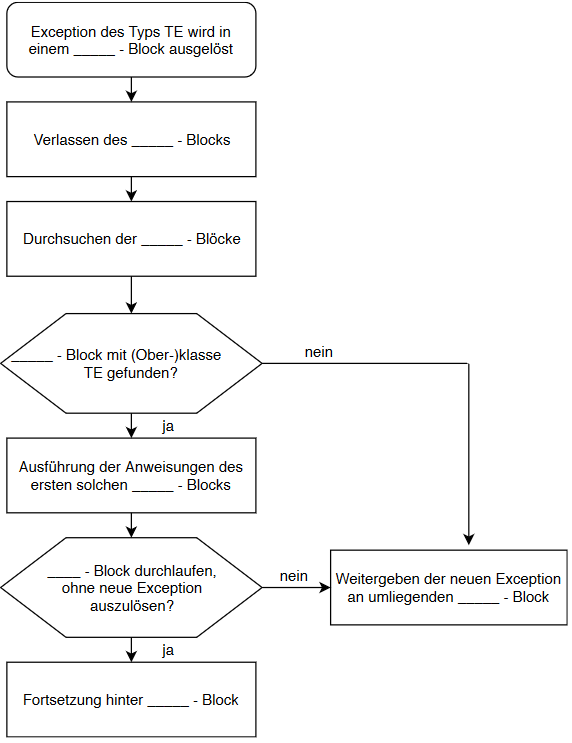
\includegraphics[width = 1\textwidth]{graphics/V4_Task.png}
    \end{minipage}

    \clearpage

    \begin{solution}
        \begin{figure}[h]
            \centering
            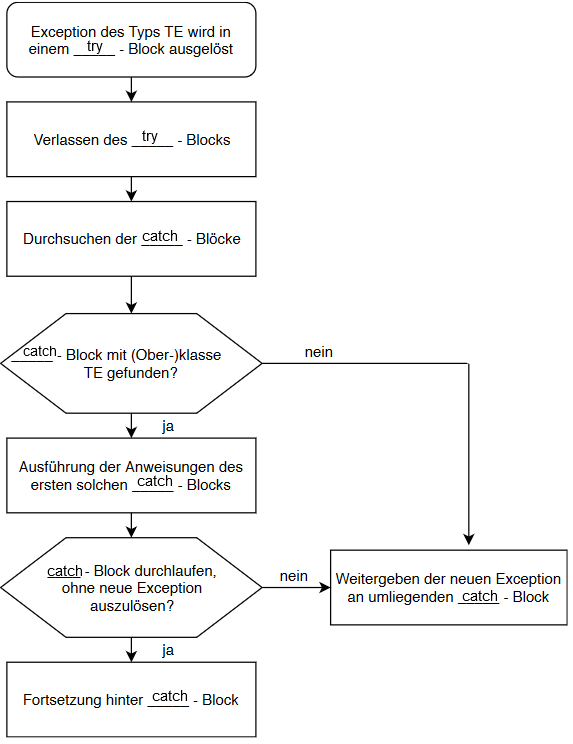
\includegraphics[width = 0.7\textwidth]{graphics/V4_Solution}
        \end{figure}
    \end{solution}
\end{task}

\clearpage

\begin{task}[credit = \stars{1}{3}]{assert-Anweisungen}
    In der Vorlesung haben Sie die assert-Anweisungen kennengelernt.
    \begin{enumerate}
        \item Beschreiben Sie in eigenen Worten, was ein Assertion-Error ist.
        \item Schreiben Sie den nachfolgenden Codeschnipsel kompakter mittels assert-Anweisungen!
              \lstinputlisting[style = Java]{codes/V5_Task.java}
        \item  Sie wissen, dass assert-Anweisungen beim Kompilieren an- oder abgeschaltet werden können mit entsprechenden Setzungen für den Compiler. Welche Vorteile ergeben sich hieraus? Warum sollten wir sie ausschalten und nicht einfach auch im realen Einsatz des Programms immer eingeschaltet mitlaufen lassen?
    \end{enumerate}

    \begin{solution}
        \begin{solution}
            \begin{enumerate}
                \item Ein Assertion-Error ist ein Fehler, der so gewichtig ist, dass er mit Fehlerbehandlung nicht zu retten ist, deshalb soll das Programm dann sofort abgebrochen werden. Ein solcher Fehler wird mit der \textcolor{keywordcolor}{assert}-Anweisung oder mit \code{AssertionError} geworfen.
                \item\hfill
                      \lstinputlisting[style = Java]{codes/V5_Solution.java}
                \item Beim Testen des Programms sind \textcolor{keywordcolor}{assert}-Anweisung sehr hilfreich, um mögliche Fehlerquellen schnell beheben zu können. Diese sollte man jedoch im realen Einsatz des Programms ausschalten, da damit sich die Laufzeit des Programms nicht unnötig verzögert.
            \end{enumerate}
        \end{solution}
    \end{solution}
\end{task}

\clearpage

\begin{task}[credit = \stars{2}{3}]{Erster Test mittels BeforeEach}
    In dieser Aufgabe wollen wir einen Blick auf die \code{BeforeEach}-Annotation von JUnit 5 werfen. Methoden mit dieser Annotation werden \textbf{vor Beginn jedes einzelnen Tests} ausgeführt!
    \br
    Gegeben sei eine Bibliothek für Geometrie-Funktionen. Dabei betrachten wir nur die Funktion \code{triangleArea}, die den Flächeninhalt eines Dreiecks berechnet und dazu die Längen der einzelnen Seiten  (\code{a}, \code{b} und \code{c}) als \textcolor{keywordcolor}{int}-Werte übergeben bekommt.

    \begin{subtask*}{Setup vor jedem Test}
        Gegeben sei folgende Klasse \code{GeoLib}:
        \lstinputlisting[style = Java]{codes/V6_1_Task.java}
        Um die Funktionen der Bibliothek verwenden zu können, muss zunächst ein Objekt vom Typ \code{GeoLib} erzeugt werden. Hierzu können Sie den parameterlosen Standard-Konstruktor der Klasse \code{GeoLib} verwenden. Schreiben Sie eine entsprechend mit JUnit-Annotationen versehene Methode namens \code{setup}, die in einer Testklasse steht und die für jeden Testfall eine neue Instanz von \code{GeoLib} in dem bereits deklarierten Attribut \code{geoLib} speichert.

        \begin{solution}
            \lstinputlisting[style = Java]{codes/V6_1_Solution.java}
        \end{solution}
    \end{subtask*}

    \clearpage

    \begin{subtask*}{Testfall}
        Schreiben Sie mindestens drei JUnit-Tests, die überprüfen, ob die Methode \code{triangleArea} für verschiedene Dreiecke korrekt arbeitet. Mindestens ein Testdreieck sollte dabei auch entartet sein.

        \begin{solution}
            \lstinputlisting[style = Java]{codes/V6_2_Solution.java}
        \end{solution}
    \end{subtask*}
\end{task}

\clearpage

\begin{task}[credit = \stars{2}{3}]{Fehlertypen}
    In der Vorlesung haben Sie kennengelernt, dass man Fehler in Programmen in zwei Kategorien einteilen kann. Es wurde unterschieden zwischen Kompilierzeitfehlern und Laufzeitfehlern.
    \begin{enumerate}[label = (\arabic*)]
        \item Beheben Sie im folgenden Codeausschnitt alle Kompilierzeitfehler:
              \lstinputlisting[style = Java]{codes/V7_Part01_Task.java}
        \item Was passiert generell beim Aufruf der Methode \code{reverseArray}? Warum kann der Code auch ohne vorhandene Kompilierzeitfehler nicht fehlerfrei ausgeführt werden? Was müsste man beheben um den Code ausführbar zu machen?
        \item Das Programm läuft zwar jetzt fehlerfrei, das Ergebnis entspricht aber noch nicht dem gewünschten Ergebnis (Array soll umgedreht werden). Beheben Sie alle fehlerhaften Stellen im Code, um das gewünschte Ergebnis zu erreichen.
    \end{enumerate}

    \clearpage

    \begin{solution}
        \begin{enumerate}[label = (\arabic*)]
            \item\hfill
                  \lstinputlisting[style = Java]{codes/V7_Part01_Solution.java}
                  \begin{itemize}
                      \item Zeile 1: \textcolor{keywordcolor}{throws} statt \textcolor{keywordcolor}{throw}
                      \item Zeile 2: \code{source.length} statt \code{source.length()}
                      \item Zeile 19: \code{Exception e}: \code{e} fehlt
                  \end{itemize}

                  \clearpage

            \item
                  \begin{itemize}
                      \item Beschreibung:
                            \newline
                            Die Methode reverseArray hat die Funktionalität ein Array in umgekehrter Reihenfolge auszugeben. Dabei wird eine Variable, welche die Länge des Arrays zwischengespeichert, zwei Laufzähler eingerichtet und das zurückzugebende Array wird deklariert. Im \textcolor{keywordcolor}{try}-Block wird das zurückzugebende Array initialisiert und die \textcolor{keywordcolor}{while}-Schleife ist für das invertieren zuständig. Wird eine \code{IndexOutOfBoundsException} oder eine Exception geworfen, so wird diese gefangen und eine Nachricht wird auf der Konsole ausgegeben.
                      \item Fehler:
                            \newline
                            Der Code wird ohne Kompilierfehler nicht durchgehen, da
                            \begin{enumerate}
                                \item Zeile 5: \code{j} zeigt auf das letzte Element des Arrays und dieser befindet sich am Index \code{length - 1}
                                \item Zeile 12 + 13: Zählvariaben wurden falsch gesetzt und somit eine \code{IndexOutOfBoundsException} geworfen wird.
                            \end{enumerate}
                  \end{itemize}
                  \lstinputlisting[style = Java]{codes/V7_Part02_Solution.java}

                  \clearpage

            \item Das Problem ist, dass in der Zeile 23 und 24 das Ergebnis überschrieben wird, welche wir vorher berechnet haben.
                  \lstinputlisting[style = Java]{codes/V7_Part02_Solution.java}
                  \begin{itemize}
                      \item Zeile 3: \code{inverted} wurde mit dem Wert \textcolor{keywordcolor}{null} initialisiert, da die Methode in jedem Fall einen Wert zurückgeben muss.
                      \item Zeile 23 und 24 wurden entfernt.
                  \end{itemize}
        \end{enumerate}
    \end{solution}
\end{task}

\clearpage

\begin{task}[credit = \stars{2}{3}]{Testen mit JUnit - Qualitätskontrolle}
    Wir wollen ein neues System zur Qualitätskontrolle in einer Produktionskette testen. Hierzu gibt es eine Klasse \code{ProductLineManagement}, die Güter (Typ \code{Product}) herstellt. Ihre Tests sollen nun prüfen, ob dies schnell genug und hinreichend gut erfolgt. Die Maschinen garantieren dabei immer eine Mindestqualität von \(89\) (\(= 89\%\) der optimalen Qualität)
    \br
    Die Qualität wird gemessen auf einer Skala von \(0\) (defekt) bis \(100\) (perfekt).
    \br
    Die Testklasse deklariert ein Attribut \textcolor{keywordcolor}{static} \code{ProductLineManagement plm}, auf das Sie zugreifen können.

    \begin{subtask*}{Setup-Methode}
        Vor jedem Test muss die (sehr komplexe) Produktionskette initialisiert werden. Dies erfolgt durch den Aufruf des Konstruktors der Klasse \code{ProductLineManagement} mit dem Namen der Firma als \code{String}. Den Firmennamen dürfen Sie beliebig wählen. Geben Sie eine mit JUnit-Annotationen versehene öffentlich sichtbare Methode an, die diese Initialisierung vor jedem Test durchführt.

        \begin{solution}
            \lstinputlisting[style = Java]{codes/V8_1_Solution.java}
        \end{solution}
    \end{subtask*}

    \begin{subtask*}{Normalfall}
        Schreiben Sie einen Test für eine normale Produktion. Hierbei soll ein einziger  Artikel \code{normalProduct} durch die Methode \code{Product} \code{produce(String)} der Klasse \code{ProductLineManagement} (siehe oben) produziert werden. Stellen Sie sicher, dass  der gelieferte Artikel nicht \textcolor{keywordcolor}{null} ist und eine Mindestqualität - abfragbar via \code{getQuality()} - von \(89\) besitzt. Als Titel des Artikels können Sie einen beliebigen \code{String} angeben.

        \begin{solution}
            \lstinputlisting[style = Java]{codes/V8_2_Solution.java}
        \end{solution}
    \end{subtask*}

    \clearpage

    \begin{subtask*}{Behandlung von Exceptions}
        Schreiben Sie nun einen weiteren Test, der auch wie im vorherigen Aufgabenteil ein neues Produkt erstellt. Nur diesmal reichen Sie dieses Produkt mittels \textcolor{keywordcolor}{boolean}  \code{submit}(\code{Product}, \textcolor{keywordcolor}{int}) aus der Klasse \code{ProductLineManagement} für die Qualitätskontrolle ein. Wurde die gewünschte Qualität erreicht, liefert die Methode \textcolor{keywordcolor}{true},  andernfalls  wirft  die  Methode eine \code{InsufficientQualityException}.
        \br
        Testen Sie das Verhalten und das Auftreten der Exception mit einem Produkt, indem Sie dieses einmal auf die (garantierte) Mindestqualität von \(89\) und einmal auf die unerreichbare Qualität von \(101\) testen.

        \begin{solution}
            \lstinputlisting[style = Java]{codes/V8_3_Solution.java}
        \end{solution}
    \end{subtask*}
\end{task}

\clearpage

\begin{task}[credit = \stars{2}{3}]{Testen: Racket und Java}
    Sie haben nun sowohl das Testen in Java mittels JUnit, als auch das Testen in Racket mittels Checks kennengelernt. In dieser Aufgabe sollen Sie zuerst eine Problemstellung in beiden Sprachen lösen und anschließend Ihre Implementierungen testen.
    \br
    Gegeben ist eine Zahlenliste. In Racket ist diese als Liste von \code{numbers} gegeben, in Java als Array von Typ \textcolor{keywordcolor}{int}[]. Außerdem sind zwei Parameter \code{lower} und \code{upper} gegeben. Ziel ist es, alle Werte aus der Zahlenliste zu sortieren, welche nicht zwischen diesen beiden Grenzwerten \code{lower} und \code{upper} liegen (jeweils exklusive).
    \br
    Ergänzen Sie die beiden untenstehenden Codeausschnitte und Verträge, um diese Problemstellung zu lösen.
    \lstinputlisting[style = Racket]{codes/V9_Part01_Task.rkt}
    \lstinputlisting[style = Java]{codes/V9_Part02_Task.java}
    Sollte der Parameter \code{lower} dabei größer als der Parameter \code{upper} sein, so soll in Java eine
    \newline
    \code{LowerBiggerThanUpperException}
    \newline
    geworfen werden. Ergänzen Sie dies in Ihrer Implementierung.
    \br
    In Racket haben Sie die Möglichkeit einen Fehler auszulösen. Dies geschieht über den Befehl (\textcolor{keywordcolor}{error} \code{msg}), wobei \code{msg} ein \code{String} mit der gewünschten Fehlermeldung ist. Konventionsmäßig einigen wir uns darauf, dass wir bei \code{msg} zuerst den Funktionsnamen nennen, gefolgt von einem Doppelpunkt und einer Beschreibung des Fehlers. Lösen Sie äquivalent zur \code{LowerBiggerThanUpperException} auch in der Racketfunktion einen Fehler für diesen Fall aus.
    \br
    Testen Sie abschließend die beiden Implementierungen mit jeweils 3 Tests. Ein Test sollte dabei das korrekte Werfen der Fehlermeldung testen.

    \clearpage

    \begin{solution}
        \lstinputlisting[style = Java]{codes/V9_Part01_Solution.java}

        \clearpage

        \lstinputlisting[style = Java]{codes/V9_Part02_Solution.java}

        \clearpage

        \lstinputlisting[style = Java]{codes/V9_Part03_Solution.java}

        \clearpage

        \lstinputlisting[style = Racket]{codes/V9_Solution.rkt}
    \end{solution}
\end{task}

\clearpage

\begin{task}[credit = \stars{2}{3}]{Exceptionklassen}
    \begin{subtask}
        Schreiben Sie eine \textcolor{keywordcolor}{public}-Klasse \code{MyException}, die von \code{Exception} erbt. Der Konstruktor dieser Klasse hat einen Parameter \code{str} vom  Typ \code{String} und einen Parametern vom Typ \textcolor{keywordcolor}{int}. Ein Objekt von \code{MyException} hat  ein \textcolor{keywordcolor}{private}-Attribut \code{message} vom  Typ \code{String}. Der Konstruktor weist \code{message} die Konkatenation aus beiden Parametern zu. Die \textcolor{keywordcolor}{public}-Methode \code{getMessage} von \code{Exception} soll so überschrieben werden, dass \code{message} zurückgeliefert wird.

        \begin{solution}
            \lstinputlisting[style = Java]{codes/V10_1_Solution.java}
        \end{solution}
    \end{subtask}

    \begin{subtask}
        Schreiben Sie eine \textcolor{keywordcolor}{public}-Klasse \code{X} mit einer \textcolor{keywordcolor}{public}-Klassenmethode \code{km}, die einen \textcolor{keywordcolor}{int}-Parameter \code{n} hat, \textcolor{keywordcolor}{int} zurückliefert und  potentiell \code{MyException} wirft. Und zwar wirft \code{km} eine \code{MyException} mit \grqq n cannot be negative\grqq{} und \code{n} als Parameterwerten, wenn negativ ist. Andernfalls liefert \code{km} das Quadrat von \code{n} zurück.

        \begin{solution}
            \lstinputlisting[style = Java]{codes/V10_2_Solution.java}
        \end{solution}
    \end{subtask}

    \clearpage

    \begin{subtask}
        Schreiben Sie eine \textcolor{keywordcolor}{public}-Klasse \code{Y} mit einer \textcolor{keywordcolor}{public}-Objektmethode \code{m}, die einen \textcolor{keywordcolor}{int}-Parameter \code{n} hat und \textcolor{keywordcolor}{int} zurückliefert. Diese Methode ruft \code{km} von \code{X} mit \code{n} auf, ohne ein Objekt von \code{X} dafür einzurichten, und liefert das Ergebnis von \code{km} zurück. Sollte \code{km} eine \code{Exception} werfen, dann soll die Botschaft der \code{Exception} auf dem Bildschirm ausgegeben werden.

        \begin{solution}
            \lstinputlisting[style = Java]{codes/V10_3_Solution.java}
        \end{solution}
    \end{subtask}
\end{task}

\clearpage

\begin{task}[credit = \stars{3}{3}]{Welcher Belag darf es sein?}
    Schreiben Sie eine Klasse \code{NoBreadException} welche von \code{Exception} erbt, im Konstruktor einen Parameter \code{String} \code{topping} erhält und damit den Konstruktor der Basisklasse mit der Konkatenation \textcolor{stringcolor}{\grqq There is no bread, only\grqq} + \code{topping} aufruft.
    \br
    Schreiben Sie dann ein Functional Interface namens \code{Lunch}. Dieses enthält die funktionale Methode \code{String}
    \newline
    \code{getTopping(String s)}, welche eine \code{NoBreadException} wirft.
    \br
    Initialisieren Sie nun das Functional Interface \code{Lunch} durch einen Lambda-Ausdruck. Geprüft werden soll, ob der \code{String} ein korrektes Sandwich ist. Dabei besteht ein korrektes Sandwich aus zweimal dem Substring \textcolor{stringcolor}{\grqq bread\grqq} und einem Topping dazwischen. Korrekte Sandwiches sind also beispielsweise \textcolor{stringcolor}{\grqq breadtunabread\grqq}oder \textcolor{stringcolor}{\grqq breadabcdefgbread\grqq}. Vordem ersten \textcolor{stringcolor}{\grqq bread\grqq} und nach dem zweiten \textcolor{stringcolor}{\grqq bread\grqq} darf kein Substring  mehr stehen. Zurückgegeben werden soll immer das Topping, also der Substring zwischen den beiden \textcolor{stringcolor}{\grqq bread\grqq}'s. Das Topping muss dabei nicht \glqq sinnvoll\grqq{}  sein, sondern irgendein beliebiger \code{String}. Ist kein Brot vorhanden, so soll eine \code{NoBreadException} mit dem alleinigen Topping geworfen werden.
    \br
    Sie dürfen davon ausgehen, dass niemals nur eine Brotscheibe verwendet wird, sondern entweder zwei oder keine.

    \begin{solution}
        \lstinputlisting[style = Java]{codes/V11_Part01_Solution.java}
        \lstinputlisting[style = Java]{codes/V11_Part02_Solution.java}
        \lstinputlisting[style = Java]{codes/V11_Part03_Solution.java}
    \end{solution}
\end{task}

\clearpage

\begin{task}[credit = \stars{3}{3}]{Arrays, Exceptions und Vererbung}
    \begin{subtask*}{Klasse X}
        \label{task:12.1}
        Gegeben sei die folgende Klasse:
        \lstinputlisting[style = Java]{codes/V12_1_Task.java}
        Wir benutzen das Array, auf das \code{a} verweist, um \textcolor{keywordcolor}{int}-Werte zu speichern. Im Array, auf das \code{writable} verweist, wird festgehalten ob ein \textcolor{keywordcolor}{int}-Wert in \code{a} überschrieben werden darf, oder nicht. Der \textcolor{keywordcolor}{int}-Wert \code{a[i]} darf überschrieben werden, wenn \code{writable[i]} == \textcolor{keywordcolor}{true}. Sie können davon ausgehen, dass beide Arrays der Klasse \code{X} immer die gleiche Länge besitzen, sodass die Indizes der beiden Arrays übereinstimmen.
        \br
        Implementieren Sie den Konstruktor der Klasse \code{X}, dieser bekommt einen \textcolor{keywordcolor}{int}-Parameter übergeben und initialisiert die Arrays \code{a} und \code{writable} mit der gleichen Länge, dabei soll jeder Wert im Array \code{writable} mit \textcolor{keywordcolor}{true} initialisiert werden. Die Länge beider Arrays entsprechen hier dem Wert des übergebenen Parameters. Erweitern Sie nun die Klasse um eine \textcolor{keywordcolor}{public}-Methode \code{save}. Die Methode liefert nichts zurück, bekommt einen \textcolor{keywordcolor}{int}-Parameter übergeben und speichert den übergebenen Parameter am kleinsten freien Index im Array \code{a} ab, an dem ein Wert nach aktueller Definition von \code{writable} überschrieben werden darf. Zusätzlich setzt sie den entsprechenden Wert im Array \code{writable} auf \textcolor{keywordcolor}{false}. Darf kein Wert überschrieben werden, so soll die Methode eine \code{ArrayStoreException} mit der Nachricht \textcolor{stringcolor}{\grqq no free space left\grqq} werfen.

        \clearpage

        \begin{solution}
            \lstinputlisting[style = Java]{codes/V12_1_Solution.java}
        \end{solution}
    \end{subtask*}

    \clearpage

    \begin{subtask*}{Klasse Y}
        Schreiben Sie nun eine Klasse \code{Y}, die von der Klasse \code{X} aus Aufgabe \hyperref{task:12.1}{V12.1} erbt. Die Klasse soll die Methode \code{save} der Oberklasse überschreiben. Die Methode liefert nichts zurück, bekommt einen \textcolor{keywordcolor}{int}-Parameter übergeben und soll mit diesem Parameter die Methode \code{save} der Oberklasse aufrufen. Wird dabei eine \code{ArrayStoreException} geworfen, so soll diese abgefangen werden. Ist dies der Fall, so sollen die beiden Arrays \code{a} und \code{writable} um ihre aktuelle Länge erweitert werden, um dann anschließend den übergebenen Parameter mittels der Methode \code{save} abspeichern zu können. Die bereits gespeicherten Werten in den beiden Arrays dürfen bei der Erweiterung nicht verloren gehen.

        \begin{solution}
            \lstinputlisting[style = Java]{codes/V12_2_Solution.java}
        \end{solution}
    \end{subtask*}
\end{task}
\end{document}
